\documentclass[12pt,]{article}
\usepackage{lmodern}
\usepackage{setspace}
\setstretch{1.2}
\usepackage{amssymb,amsmath}
\usepackage{ifxetex,ifluatex}
\usepackage{fixltx2e} % provides \textsubscript
\ifnum 0\ifxetex 1\fi\ifluatex 1\fi=0 % if pdftex
  \usepackage[T1]{fontenc}
  \usepackage[utf8]{inputenc}
\else % if luatex or xelatex
  \ifxetex
    \usepackage{mathspec}
  \else
    \usepackage{fontspec}
  \fi
  \defaultfontfeatures{Ligatures=TeX,Scale=MatchLowercase}
    \setmainfont[]{Times New Roman}
    \setsansfont[]{Times New Roman}
\fi
% use upquote if available, for straight quotes in verbatim environments
\IfFileExists{upquote.sty}{\usepackage{upquote}}{}
% use microtype if available
\IfFileExists{microtype.sty}{%
\usepackage{microtype}
\UseMicrotypeSet[protrusion]{basicmath} % disable protrusion for tt fonts
}{}
\usepackage[margin=1in]{geometry}
\usepackage{hyperref}
\PassOptionsToPackage{usenames,dvipsnames}{color} % color is loaded by hyperref
\hypersetup{unicode=true,
            colorlinks=true,
            linkcolor=Maroon,
            citecolor=Blue,
            urlcolor=Blue,
            breaklinks=true}
\urlstyle{same}  % don't use monospace font for urls
\usepackage{longtable,booktabs}
\usepackage{graphicx,grffile}
\makeatletter
\def\maxwidth{\ifdim\Gin@nat@width>\linewidth\linewidth\else\Gin@nat@width\fi}
\def\maxheight{\ifdim\Gin@nat@height>\textheight\textheight\else\Gin@nat@height\fi}
\makeatother
% Scale images if necessary, so that they will not overflow the page
% margins by default, and it is still possible to overwrite the defaults
% using explicit options in \includegraphics[width, height, ...]{}
\setkeys{Gin}{width=\maxwidth,height=\maxheight,keepaspectratio}
\IfFileExists{parskip.sty}{%
\usepackage{parskip}
}{% else
\setlength{\parindent}{0pt}
\setlength{\parskip}{6pt plus 2pt minus 1pt}
}
\setlength{\emergencystretch}{3em}  % prevent overfull lines
\providecommand{\tightlist}{%
  \setlength{\itemsep}{0pt}\setlength{\parskip}{0pt}}
\setcounter{secnumdepth}{5}
% Redefines (sub)paragraphs to behave more like sections
\ifx\paragraph\undefined\else
\let\oldparagraph\paragraph
\renewcommand{\paragraph}[1]{\oldparagraph{#1}\mbox{}}
\fi
\ifx\subparagraph\undefined\else
\let\oldsubparagraph\subparagraph
\renewcommand{\subparagraph}[1]{\oldsubparagraph{#1}\mbox{}}
\fi

%%% Use protect on footnotes to avoid problems with footnotes in titles
\let\rmarkdownfootnote\footnote%
\def\footnote{\protect\rmarkdownfootnote}

%%% Change title format to be more compact
\usepackage{titling}

% Create subtitle command for use in maketitle
\providecommand{\subtitle}[1]{
  \posttitle{
    \begin{center}\large#1\end{center}
    }
}

\setlength{\droptitle}{-2em}

  \title{\vspace{1cm}Measuring political participation levels and inequality with survey data: Failed attempts*\footnote{*This is a draft. Do not quote, cite, or distribute. Funding: ``Political Voice and Economic Inequality across Nations and Time'', Poland's National Science Centre (2016/23/B/HS6/03916). \url{https://politicalinequality.org/2017/09/21/new-project-political-voice-and-economic-inequality-across-nations-and-time/}}\vspace{0.5cm}\\}
    \pretitle{\vspace{\droptitle}\centering\huge}
  \posttitle{\par}
    \author{}
    \preauthor{}\postauthor{}
      \predate{\centering\large\emph}
  \postdate{\par}
    \date{9 April, 2019\\
~\\}

\usepackage[polish, english]{babel}
\usepackage[T1]{fontenc}
\usepackage{float}
\usepackage{lmodern}
\usepackage{graphicx}
\usepackage{url}
\usepackage{array}
\usepackage{setspace}
\usepackage{graphics}
%\usepackage{amssymb}
\usepackage{amsmath}
\usepackage{longtable}
\usepackage{natbib}
\usepackage{pdflscape}
\usepackage{caption}
\usepackage{subcaption}
\usepackage{fullpage}
\usepackage{multicol}
\usepackage{dcolumn}
\usepackage{lscape}
\usepackage{array}
\usepackage{color}
\usepackage{setspace}

\usepackage{cleveref}[2012/02/15]
\usepackage{fullpage}
\usepackage[charter]{mathdesign}
\usepackage{bm}
\usepackage{tabu}
\usepackage{wrapfig}

\usepackage{babel}
\usepackage[utf8]{inputenc}
\DeclareUnicodeCharacter{0229}{\k{e}}

\crefformat{footnote}{#2\footnotemark[#1]#3}
\usepackage{color}
\usepackage{hyperref}

\newenvironment{tightcenter}{%
  \setlength\topsep{0pt}
  \setlength\parskip{0pt}
  \begin{center}
}{%
  \end{center}
}

%\setstretch{1.1}
% Dutch style of paragraph formatting
\parskip 5pt
\makeatletter
% Separation between lines
\doublerulesep 1pt

\usepackage[table]{xcolor}

\definecolor{lightred}{rgb}{0.7,0,0}
\definecolor{darkgreen}{rgb}{0,0.8,0}
\definecolor{lightblue}{rgb}{0,0,0.7}

\hypersetup{colorlinks,
  linkcolor = lightred,
  filecolor = lightred,
  urlcolor = lightblue,
  citecolor = lightred}

% Spaces in bibliography
\let\oldthebibliography=\thebibliography
\let\endoldthebibliography=\endthebibliography
\renewenvironment{thebibliography}[1]{%
  \begin{oldthebibliography}{#1}%
    \setlength{\parskip}{0ex}%
    \setlength{\itemsep}{0.1ex}%
  }%
  {%
  \end{oldthebibliography}%
}

\usepackage{array}
\newcolumntype{L}[1]{>{\raggedright\let\newline\\\arraybackslash\hspace{0pt}}m{#1}}
\newcolumntype{C}[1]{>{\centering\let\newline\\\arraybackslash\hspace{0pt}}m{#1}}
\newcolumntype{R}[1]{>{\raggedleft\let\newline\\\arraybackslash\hspace{0pt}}m{#1}}

\setlength{\parindent}{0pt} % no indentation
\usepackage{booktabs}
\usepackage{longtable}
\usepackage{array}
\usepackage{multirow}
\usepackage{wrapfig}
\usepackage{float}
\usepackage{colortbl}
\usepackage{pdflscape}
\usepackage{tabu}
\usepackage{threeparttable}
\usepackage{threeparttablex}
\usepackage[normalem]{ulem}
\usepackage{makecell}
\usepackage{xcolor}

\usepackage{dcolumn}
\usepackage{color}

\begin{document}
\maketitle
\begin{abstract}
\noindent\setstretch{1}This report documents the work on constructing measures of levels and inequality of political participation on the basis of existing cross-national survey data. Altogether six ideas were tested: (1) index of political participation as a continuous variable and its inequality, (2) entropy of participation profiles, (3) ratio measures of the proportion of participants in various activities to the proportion of non-participants, (4) country ranks by activity type, (5) canonical correlations between a set of basic socio-demographics and a set of variables on participation in different activities, and (6) re-weighting samples to match the age, gender, and education distribution. The empirical strategy involved comparing sample statistics from two surveys carried out at more or less the same time in the same countries as part of two survey projects -- the European Social Survey Round 7 and the International Social Survey Programme Round 2014, to verify whether the given measure of the level or inequality of participation is consistent across projects. The general conclusion is that the aggregate measures of participation or its inequality differ between surveys carried out in different projects in the same countries and years, some of the differences are very large, and they cannot be explained by the sample composition. This questions the comparability of aggregate measures derived from cross-national survey data. \vspace{.8cm}
\end{abstract}

\clearpage

\renewcommand{\baselinestretch}{0.5}\normalsize
\tableofcontents
\renewcommand{\baselinestretch}{1.1}\normalsize

\clearpage

\hypertarget{the-problem}{%
\section{The problem}\label{the-problem}}

Political participation is an important aspect of civic engagement, and the inequality of political participation might be a symptom of either unequal opportunities for participation, the cause of unequal influence over policy decisions, or both.

In theory, political participation should be easy to measure, because -- as a behavior -- it is observable. At the same time what constitutes political participation (and what doesn't) is not clear, different forms of behavior might become political under certain conditions, and moreover certain forms of inactivity have a political meaning, such as abstaining from voting or boycotting (i.e., abstaining form buying or using) products or services.

The goal of this exercise was to create measures of political participation and of the inequality of political participation that are: (1) based on data from cross-national survey projects, ideally primarily on items on participation in demonstrations and signing petitions, which are included in the SDR v.1 dataset, (2) comparable across countries and over time, (3) insensitive to methodological differences among surveys, including differences between sample types and especially to the design of the participation questionnaire items or batteries.

This report describes six ideas that were intended to test various properties of the survey data, the survey measurement of political participation, and the comparability of sample aggregates across surveys carried out in the same country and (more or less) at the same time. The first idea was to construct an index of political participation as a weighted sum of participation in five activities. Political participation, as a formative concept, would be defined by the five observed variables, and the measure of participation inequality would be the Gini index. The second idea was to calculate the heterogeneity of participation profiles, or sets of activities in which individuals participate or not participate.

The third idea was to calculate the ratio of proportions of individuals who vote in elections and also engage in other forms of participation divided by the proportion of individuals who do none. The fourth idea involved ranking countries by their level of participation in separate activities to see if these rankings are consistent across ESS and ISSP. The fifth idea was about the extent to which participation is associated with age, gender, and education, and involved calculating canonical correlations of the set of socio-demographics and a set of participation dummies. Finally, the sixth idea was about adjusting the sample composition to match age, gender, and education distributions, to see if this brings close the levels of participation recorded by both projects.

\hypertarget{data}{%
\section{Data}\label{data}}

Data come from the \href{https://www.europeansocialsurvey.org/data/round-index.html}{European Social Survey Round 7} and the \href{https://www.gesis.org/issp/modules/issp-modules-by-topic/citizenship/2014/}{International Social Survey Programme Wave 2014 (Citizenship II)}, both carried out in or around 2014. The ESS covered 21 countries and the ISSP - 34. Eighteen countries were surveyed in both projects: Austria, Belgium Switzerland, Czechia, Germany, Denmark, Spain, Finland, France, Hungary, Israel, Lithuania, Netherlands, Norway, Poland, Sweden, and Slovenia.

In both waves respondents were asked about participation in political activities. It is worth mentioning that while all ESS waves contain participation batteries with only small changes from wave to wave, most ISSP modules do not ask about participation in multiple activities with the exception of the Citizenship module (2004 and 2014).

\hypertarget{ess7-political-participation-questions}{%
\subsection{ESS/7: Political participation questions}\label{ess7-political-participation-questions}}

There are different ways of trying to improve things in {[}country{]} or help prevent things from going wrong. During the last 12 months, have you done any of the following?\\
Have you:\\
B11 contacted a politician, government or local government official?\\
B12 worked in a political party or action group?\\
B13 worked in another organisation or association?\\
B14 worn or displayed a campaign badge/sticker?\\
B15 signed a petition?\\
B16 taken part in a lawful public demonstration?\\
B17 boycotted certain products?

\hypertarget{issp2014-political-participation-questions}{%
\subsection{ISSP/2014: Political participation questions}\label{issp2014-political-participation-questions}}

Here are some different forms of political and social action that people can take. Please indicate, for each one,\\
- whether you have done any of these things in the past year,\\
- whether you have done it in the more distant past,\\
- whether you have not done it but might do it,\\
- or have not done it and would never, under any circumstances, do it.\\
13. Signed a petition\\
14. Boycotted, or deliberately bought, certain products for political, ethical or environmental reasons\\
15. Took part in a demonstration\\
16. Attended a political meeting or rally\\
17. Contacted, or attempted to contact, a politician or a civil servant to express your views\\
18. Donated money or raised funds for a social or political activity\\
19. Contacted or appeared in the media to express your views\\
20. Expressed political views on the internet\\
\ldots{}\\
People sometimes belong to different kinds of groups or associations. For each type of group, please indicate whether you,\\
- belong and actively participate,\\
- belong but don't actively participate,\\
- used to belong but do not any more,\\
- or have never belonged to it.\\
23. A political party\\
24. A trade union, business, or professional association\\
25. A church or other religious organization\\
26. A sports, leisure or cultural group\\
27. Another voluntary association

The table below shows the availability and overlap of participation items in ESS/7 and ISSP/2014.

\begin{table}[H]

\caption{\label{tab:ind-table}Availability of participation items in ESS/7 and ISSP/2014.}
\centering
\resizebox{\linewidth}{!}{
\fontsize{10}{12}\selectfont
\begin{tabular}{lll}
\toprule
Indicator & ESS/7 & ISSP/2014\\
\midrule
\rowcolor{gray!6}  petition & Petition & Petition\\
boycott & Boycott & Boycott or buycott\\
\rowcolor{gray!6}  demonstration & Lawful public demonstration & Demonstration\\
demonstration &  & Rally\\
\rowcolor{gray!6}  contact & Contact politician & Contact politician or attempted contact\\
\addlinespace
 &  & Donation\\
\rowcolor{gray!6}   &  & Media contact or appearance\\
 &  & Express views on the internet\\
\rowcolor{gray!6}   & Display badge or sticker & \\
party & Work in political party & Belong to political party\\
\addlinespace
\rowcolor{gray!6}  party & Work in organization & \\
party &  & Belong to trade union, business, or professional association\\
\rowcolor{gray!6}   &  & Belong to church or other religious organization\\
 &  & Belong to sports, leisure or cultural group\\
\rowcolor{gray!6}   &  & Belong to another voluntary association\\
\bottomrule
\end{tabular}}
\end{table}

\hypertarget{selected-activities}{%
\subsection{Selected activities}\label{selected-activities}}

Five activities have been selected as part of non-electoral political participation: signing petitions, boycotting, demonstrations (includes rallies in ISSP), contacting politicians, and work (active participation in ISSP) in political parties (or other organizations - ESS, or trade unions - ISSP). Only participation in the last year / 12 months was coded as 1. Table 1 shows which source variables were used as indicators of these activities.

Both ESS/7 and ISSP/2014 also ask about voting in last elections. Voting is considered separately from non-electoral political participation, and is only used in the third measure.

\hypertarget{country-levels-of-participation-in-single-activities}{%
\subsection{Country levels of participation in single activities}\label{country-levels-of-participation-in-single-activities}}

Thanks to the country overlap, it is possible to compare participation levels in the same countries from different projects. In both cases samples have been restricted to respondents aged 18-65. Appropriate case weights (\texttt{pspwgh} in ESS and \texttt{WEIGHT} in ISSP) were applied.

The scatter plot shows participation levels by country. Each dot is a country. Colors indicate the type of activity. In most cases the points are reasonably close to the 45-degree line. The only exception is work/active membership in political parties and other organizations, which might result from the differences in source variables and in the construction of the ``party'' indicator. Levels of contacting politicians are systematically higher in ESS than in ISSP, which is surprising given that the ISSP question also included ``attempted contact''.

\begin{figure}[H]

{\centering 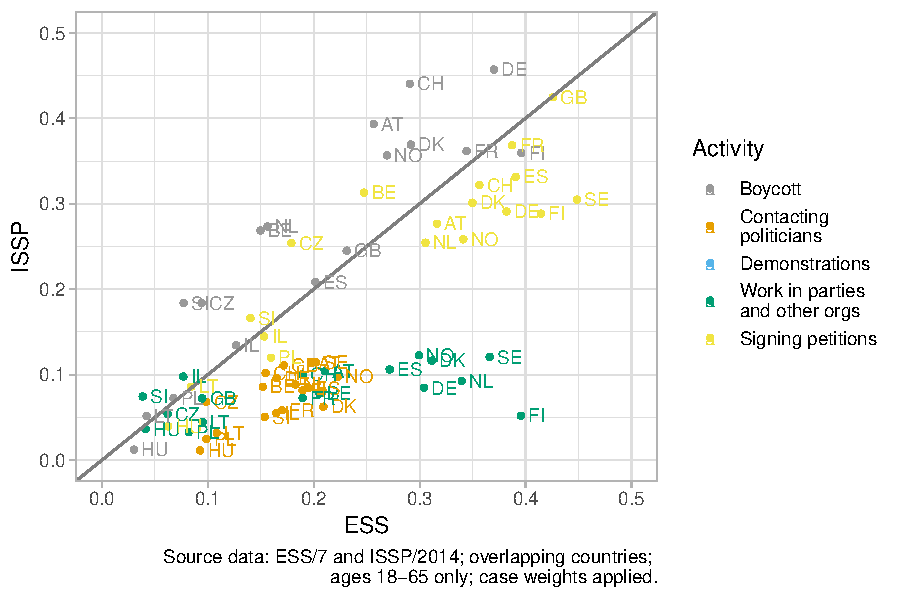
\includegraphics{report_files/figure-latex/part-rate-dot-plot-1} 

}

\caption{Participation levels in single activities}\label{fig:part-rate-dot-plot}
\end{figure}

\hypertarget{attempt-1-gini-index-of-the-weighted-sum-of-activities}{%
\section{Attempt 1: Gini index of the weighted sum of activities}\label{attempt-1-gini-index-of-the-weighted-sum-of-activities}}

In the first approach political participation was conceptualized as a continuous characteristic corresponding to the weighted sum of distinct activities the responded declared having participated in. Participation inequality was measured as the Gini coefficient of that participation.

\hypertarget{weighting-political-participation}{%
\subsection{Weighting political participation}\label{weighting-political-participation}}

Intuitively, when combining multiple forms of political participation in a single scale, different activities should be weighted differently to reflect either the effort needed to participate (in terms of time and/or money) or the effectiveness of participation. It is hard to calculate weights that capture either effort or effectiveness, but we seem to have agreed that less popular activities should have more weight.

Here I consider different types of weights. The first three are functions of the participation level:
- The probit of the complement of the participation level: \(probit(1 - p_{i,j})\),\\
- The natural log of the reciprocal of the participation level: \(ln(1 / p_{i,j})\),\\
- The square root of the reciprocal of the participation level: \(1/\sqrt{p_{i,j}}\),

where \(p_{i,j}\) is the level of participation in activity \emph{i} in country \emph{j}. The graph below shows how the value of the weight depends on the level of participation. In the analyses that follow I decided to drop the reciprocal of the square root because of the extremely high weights it would assign to rare activities.

\begin{figure}[H]

{\centering 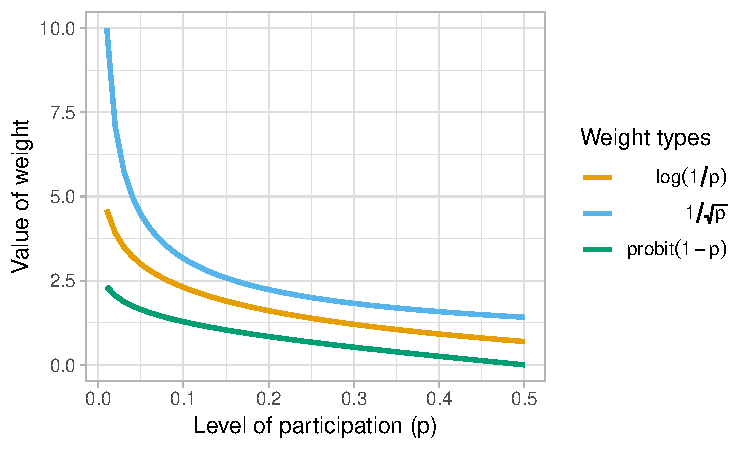
\includegraphics{report_files/figure-latex/weights-1} 

}

\caption{Weight value as function of the sample proportion}\label{fig:weights}
\end{figure}

The two remaining types of weights do not take participation levels into account:\\
- Ranks according to the estimated effort associated with each activity, in descending order. The rank weights were assigned as follows: work in party or organization (5), participation in demonstrations (4), contacting politicians (3), signing petitions (2), and boycotting (1),\\
- Unit weights (weighted number of activities the respondent participated in).

I constructed another political participation indicator to serve as a benchmark:\\
- A dummy indicating whether the respondent took part in any of the 5 selected activities (coded 1) or if they didn't take part in any (coded 0).

\hypertarget{country-levels-of-overall-political-participation}{%
\subsection{Country levels of overall political participation}\label{country-levels-of-overall-political-participation}}

For each of the five variants of weights I calculate the Political Participation Score (PPS) for each individual. Sample means of PPS for countries that appear in both ESS and in ISSP are shown on the graph below.

\begin{figure}[H]

{\centering 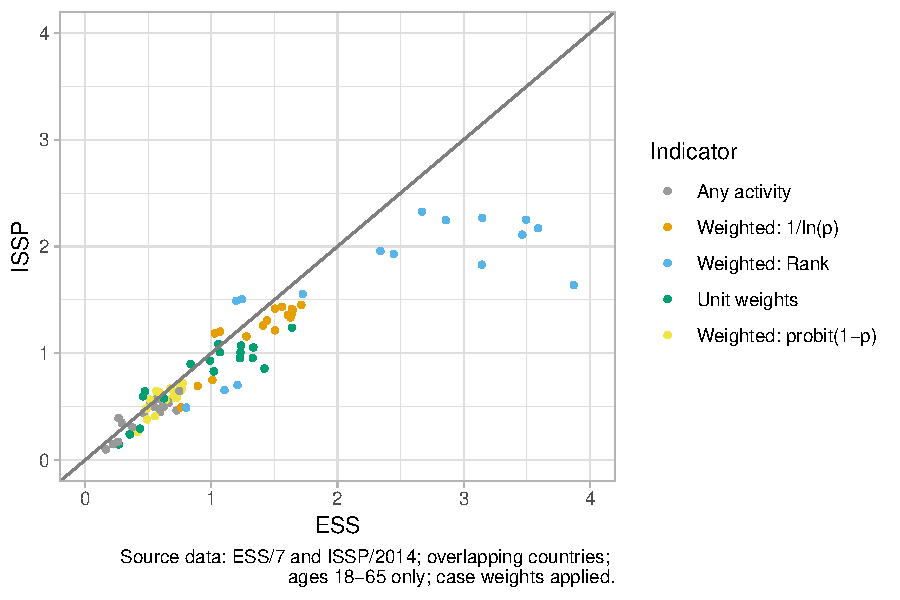
\includegraphics{report_files/figure-latex/part-level-dot-plot-1} 

}

\caption{Political participation levels by indicator type}\label{fig:part-level-dot-plot}
\end{figure}

\hypertarget{correlations-with-interest-in-politics}{%
\subsubsection{Correlations with interest in politics}\label{correlations-with-interest-in-politics}}

One way of determining which of the participation measures is best would be to analyze their association with a variable that is known to correlate with political participation. The strongest correlate of political participation is probably interest in politics, although it is not clear what correlation can be reasonably expected other than they should be positive.

Correlations between each of the PPS variants and interest in politics by country range from around 0.21 to 0.43 in the ESS, and from 0.12 and 0.44 in the ISSP. The means are around 0.3 and 0.28, respectively. The differences in correlations across the variants of PPS are very small, and do not clearly favor one or the other variant. On average, in both projects the log of inverse proportion and the unweighted sum fare a little better than the other two variants.

\hypertarget{political-participation-inequality}{%
\subsection{Political participation inequality}\label{political-participation-inequality}}

For each variant of the Political Participation Score, except for the dichotomous one, I calculated the Gini coefficient. The graph below shows the associations between Gini coefficients in countries covered by both ESS and ISSP. The dots again represent countries, but the colors now correspond to the PPS Gini variants. Overall it seems that the differences between country measurements are the smallest (dots are closest to the 45-degree line) in the case of the unweighted PPS Gini index.

\begin{figure}[H]

{\centering 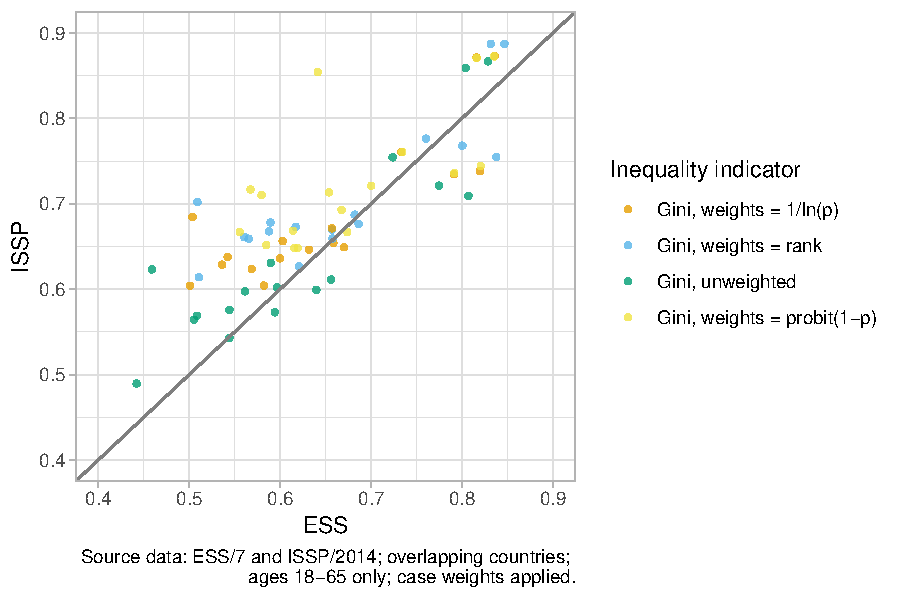
\includegraphics{report_files/figure-latex/part-gini-dot-plot-1} 

}

\caption{Political participation inequality}\label{fig:part-gini-dot-plot}
\end{figure}

\hypertarget{correlations-between-pps-levels-and-inequality}{%
\subsubsection{Correlations between PPS levels and inequality}\label{correlations-between-pps-levels-and-inequality}}

It turns out that there is an almost perfect negative correlation (around -0.96 to -0.99) between the inequality of political participation and the proportion of individuals who participated in at least one of the five activities. This suggests that the value of the Gini index is largely driven by the proportion of zeroes, i.e.~of the non-participants.

\hypertarget{attempt-2-entropy-of-political-participation-profiles}{%
\section{Attempt 2: Entropy of political participation profiles}\label{attempt-2-entropy-of-political-participation-profiles}}

The second approach to measuring the inequality of political participation follows an entirely different strategy. Instead of quantifying the amount of participation to calculate its inequality, it focuses on participation profiles, i.e.~combinations of activities individuals engage in, and calculates the heterogeneity of these profiles using information entropy.

For an ordered set of \(n\) activities, a participation profile is a vector of length \(n\) consisting of values \(0\) and \(1\), where the position of the value indicates the participation (1) or lack of participation (0) in the corresponding activity.

\begin{table}[H]

\caption{\label{tab:ess-part-profile}Creating participation profiles, example.}
\centering
\resizebox{\linewidth}{!}{
\fontsize{10}{12}\selectfont
\begin{tabular}{llllll}
\toprule
Party / organization & Demonstration & Contact politicians & Petition & Boycott & Participation profile\\
\midrule
\rowcolor{gray!6}  1 & 0 & 0 & 0 & 1 & 1 0 0 0 1\\
0 & 0 & 0 & 0 & 0 & 0 0 0 0 \vphantom{1} 0\\
\rowcolor{gray!6}  0 & 0 & 0 & 0 & 1 & 0 0 0 0 1\\
1 & 0 & 0 & 0 & 0 & 1 0 0 0 0\\
\rowcolor{gray!6}  0 & 0 & 0 & 0 & 0 & 0 0 0 0 0\\
\bottomrule
\end{tabular}}
\end{table}

While all \(2^5=32\) possible participation profiles are represented in the ESS/7 data, not all occur in all countries. For example, in Slovenia 25 profiles are represented, in France and Hungary - 26.

Entropy is calculated as the negative of the sum of the proportion in each group multiplied by the logarithm of the proportion:

\[ entropy =-\sum_{i=1}^{n} p_i log(p_i) \]
where \(p_i\) is the proportion of cases in the \(i\)-th group.

\hypertarget{correlations-between-entropy-and-pps-inequality}{%
\subsection{Correlations between entropy and PPS inequality}\label{correlations-between-entropy-and-pps-inequality}}

Entropy is low when concentration is high, so the correlation between entropy and the Gini coefficient should be negative. The graphs below show that the correlation between entropy of political participation profiles and the Gini coefficient of political participation (with unit weights) is close to -1. This again suggests that a large role is played by one dominating profile, i.e.~the non-participants.

\begin{figure}[H]

{\centering 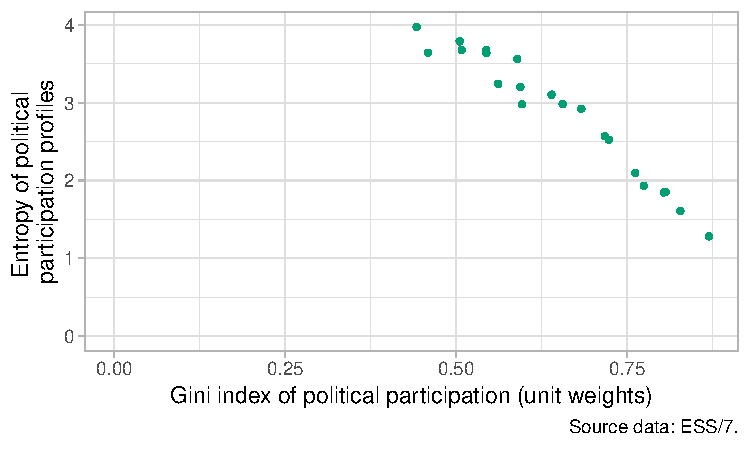
\includegraphics{report_files/figure-latex/ess-entropy-1} 

}

\caption{Gini index of political participation (unit weights) vs. Entropy of political participation profiles.}\label{fig:ess-entropy}
\end{figure}

\begin{figure}[H]

{\centering 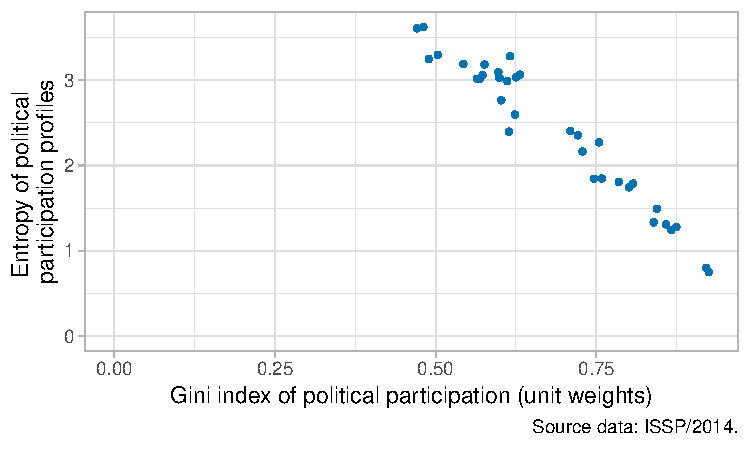
\includegraphics{report_files/figure-latex/issp-entropy-1} 

}

\caption{Gini index of political participation (unit weights) vs. Entropy of political participation profiles.}\label{fig:issp-entropy}
\end{figure}

\hypertarget{attempt-3-ratio-of-the-proportion-of-the-active-to-the-proportion-of-the-inactive}{%
\section{Attempt 3: Ratio of the proportion of the active to the proportion of the inactive}\label{attempt-3-ratio-of-the-proportion-of-the-active-to-the-proportion-of-the-inactive}}

The third attempt proposes to calculate political participation inequality as the ratio of the proportion of individuals who engaged in both non-electoral participation and voting divided by the proportion of those who did neither. Values above 1 indicate that the proportion of active individuals is higher than the proportion of inactive individuals, while values below 1 indicate the opposite.

The graphs below show these ratios for each country, separately for the ESS and the ISSP. The \textcolor{Cerulean}{blue} horizontal line separates the values below and above 1.

\begin{figure}[H]

{\centering 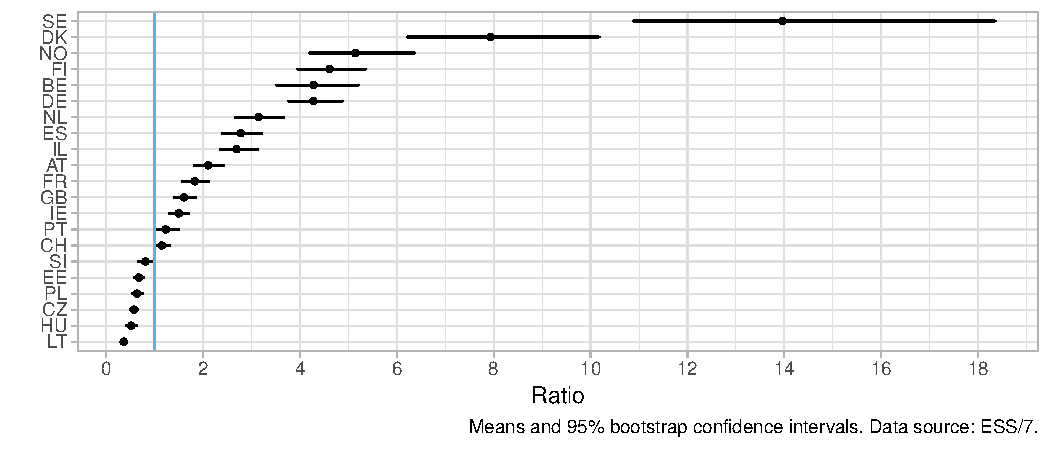
\includegraphics{report_files/figure-latex/ess-ratio-all-1} 

}

\caption{Ratio of proportion voted and participated to proportion neither voted nor participated.}\label{fig:ess-ratio-all}
\end{figure}

\begin{figure}[H]

{\centering 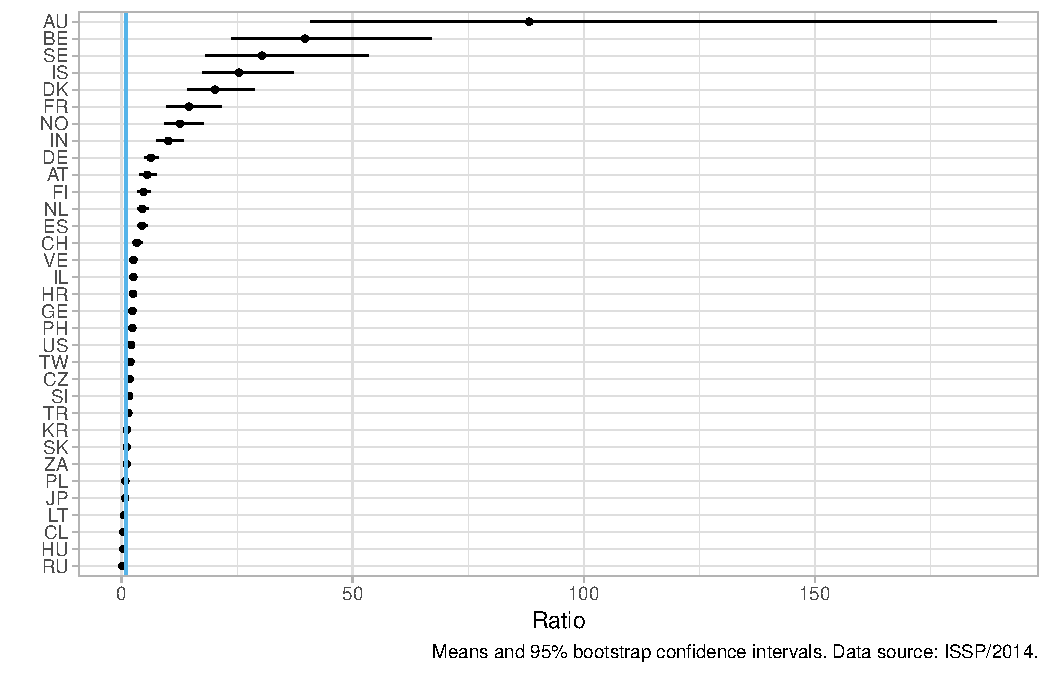
\includegraphics{report_files/figure-latex/issp-ratio-all-1} 

}

\caption{Ratio of proportion voted and participated to proportion neither voted nor participated.}\label{fig:issp-ratio-all}
\end{figure}

\hypertarget{attempt-4-country-ranks-by-activity}{%
\section{Attempt 4: Country ranks by activity}\label{attempt-4-country-ranks-by-activity}}

\begin{figure}[H]

{\centering 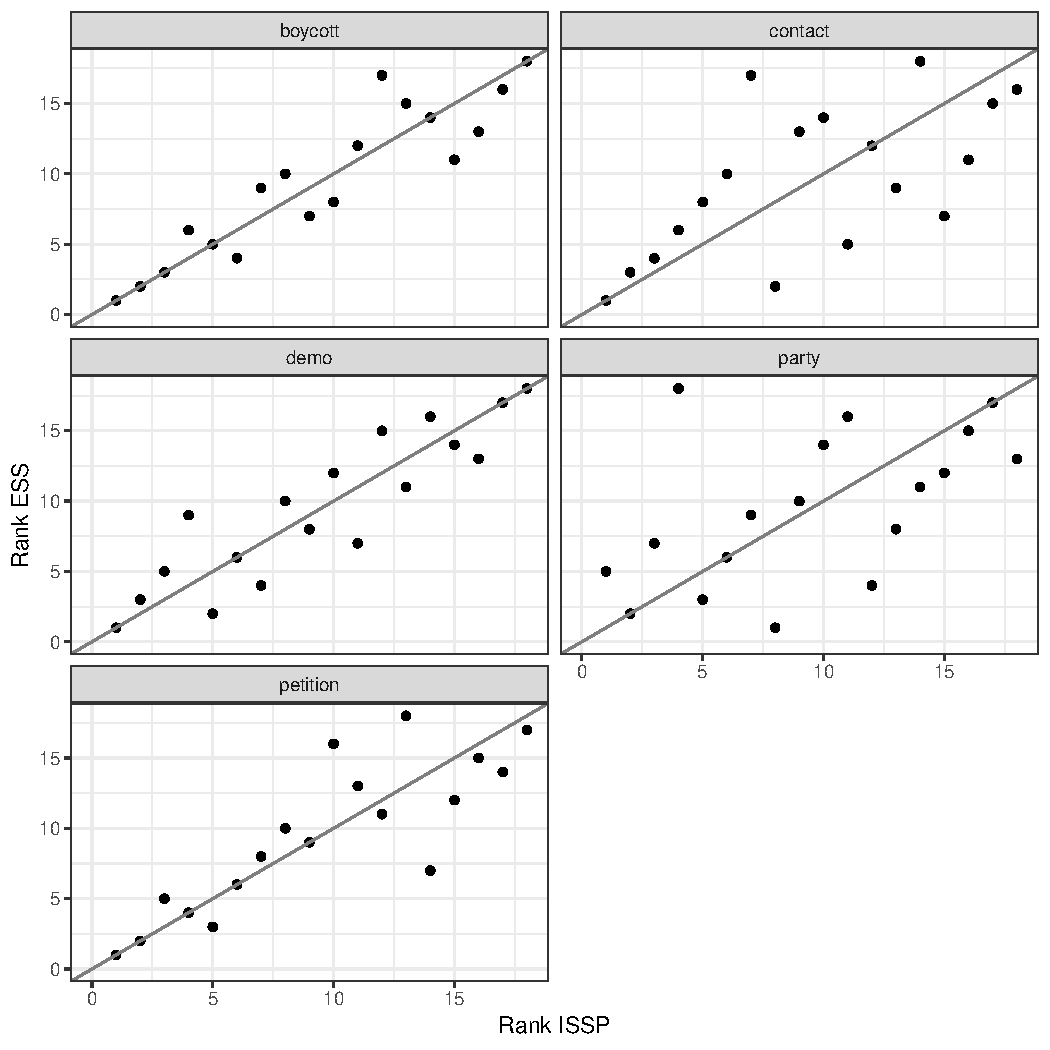
\includegraphics{report_files/figure-latex/cntry-ranks-1} 

}

\caption{Canonical correlations between participation and sociodemograhics: ESS/7 and ISSP/2014.}\label{fig:cntry-ranks}
\end{figure}

\hypertarget{attempt-5-canonical-correlations}{%
\section{Attempt 5: Canonical correlations}\label{attempt-5-canonical-correlations}}

In the second attempt a different approach was explored. The question was whether the extent to which political participation is associated with basic socio-demographic variables (age, gender, and education) varies across countries, and whether it is consistent within countries in the two survey projects, ESS and ISSP.

Canonical correlations were calculated for five binary variables corresponding to the five activities on one side, and gender, age (3 categories) and education (3 categories) on the other. Figure \ref{fig:can-cor} shows the correlation coefficients for all countries covered by both ESS and ISSP. The correlation between both series is around 0.2.

\begin{figure}[H]

{\centering 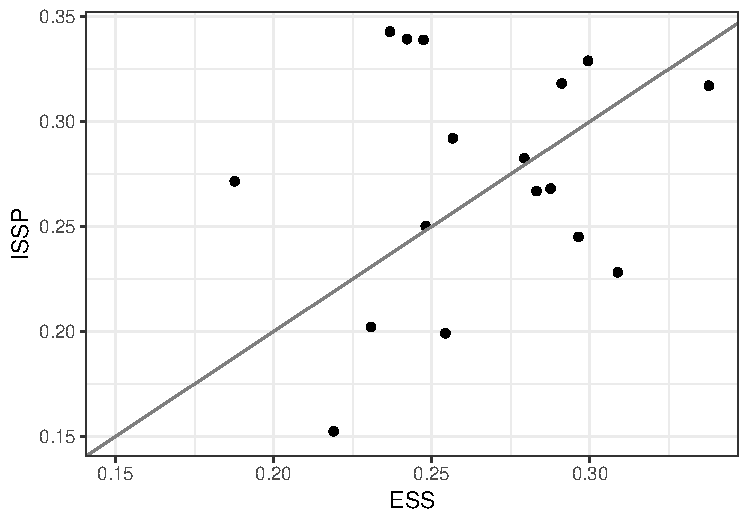
\includegraphics{report_files/figure-latex/can-cor-1} 

}

\caption{Canonical correlations between participation and sociodemograhics: ESS/7 and ISSP/2014.}\label{fig:can-cor}
\end{figure}

\hypertarget{attempt-6-sample-composition-re-weighting-samples}{%
\section{Attempt 6: Sample composition: Re-weighting samples}\label{attempt-6-sample-composition-re-weighting-samples}}

To account for possible sample composition differences, weights were calculated to adjust the gender*age*education groups in ISSP to their proportions in the ESS samples. Three age groups were considered - 18-29, 30-49, 50-65 - and three education groups - secondary, post-decondary non-tertiary, and tertiary education. Altogether this makes \(2*3*3=18\) combinations.

Table \ref{tab:sample-re-weighting} shows correlations between sample proportions in the ESS and in the (un-weighted) ISSP, and the same correlations between ESS and ISSP re-weighted to match sample proportions from the ESS. In all cases the correlations with the re-weighted data are weaker, with the largest difference for work in a political party (0.57 compared to 0.34), and smaller declines in the case of the other activities.

\begin{table}[t]

\caption{\label{tab:sample-re-weighting}Correlations between ESS and ISSP participation levels.}
\centering
\fontsize{11}{13}\selectfont
\begin{tabular}{lrr}
\toprule
Activity & ESS \& ISSP & ESS \& ISSP re-weighted\\
\midrule
\rowcolor{gray!6}  boycott & 0.929 & 0.906\\
contact & 0.727 & 0.612\\
\rowcolor{gray!6}  demo & 0.915 & 0.901\\
party & 0.565 & 0.341\\
\rowcolor{gray!6}  petition & 0.888 & 0.823\\
\bottomrule
\end{tabular}
\end{table}


\end{document}
